\documentclass[11pt,usenames,dvipsnames]{beamer}

\usetheme{CambridgeUS}
\usecolortheme{dolphin}

\usepackage{appendixnumberbeamer}
\usepackage[utf8]{inputenc}
\usepackage[T1]{fontenc}
\usepackage[french, francais]{babel}
\usepackage{array}
\usepackage{stmaryrd}
\usepackage{amsmath}
\usepackage{amsfonts}
\usepackage{amssymb}
\usepackage{galois}
\usepackage{float}
\usepackage{graphicx}
\usepackage{subfig}
\usepackage{listingsutf8}
\usepackage{lmodern}
\usepackage{caption}
\usepackage{pifont}
\usepackage{algpseudocode}
\usepackage[plain]{algorithm}
\usepackage{eqparbox}
\usepackage{syntax}
\usepackage{mdwtab}
\usepackage{hyperref}
\usepackage{tabularx}
\usepackage{fancyvrb}
\usepackage{color}%% \usepackage{color}
\definecolor{mygreen}{rgb}{0,0.6,0}
\definecolor{mygray}{rgb}{0.5,0.5,0.5}
\definecolor{mymauve}{rgb}{0.58,0,0.82}
\definecolor{OliveGreen}{RGB}{0, 182, 12}%219, 0}
\usepackage{xcolor}
\uselanguage{French}
\languagepath{French}
\usepackage{tikz}
\usetikzlibrary{calc}

\usefonttheme[onlymath]{serif}


\setbeamertemplate{itemize items}[triangle]
\setbeamertemplate{enumerate items}[square]
\setbeamertemplate{caption}[numbered]
\beamertemplatenavigationsymbolsempty

\newif\iflattersubsect


\AtBeginSection[]
{
\begin{frame}<beamer>
\tableofcontents[
  currentsection,
  sectionstyle=show/shaded,
  subsectionstyle=show/show/hide%%shaded/hide
%  \lattersubsectfalse
]
\end{frame}
}

%% \AtBeginSection[] {
%%     \begin{frame}<beamer>
%% %    \frametitle{Inhalt} %
%%     \tableofcontents[currentsection]
%%     \end{frame}
%% }
%% \setbeamertemplate{navigation symbols}{}{%
%%     \usebeamerfont{footline}%
%%     \usebeamercolor[fg]{footline}%
%%     \hspace{1em}%
%%     \insertframenumber/\inserttotalframenumber
%% }
\lstset{ %
  backgroundcolor=\color{white},   % choose the background color; you must add \usepackage{color} or \usepackage{xcolor}
  basicstyle=\footnotesize,        % the size of the fonts that are used for the code
  breakatwhitespace=false,         % sets if automatic breaks should only happen at whitespace
  breaklines=true,                 % sets automatic line breaking
  captionpos=b,                    % sets the caption-position to bottom
  commentstyle=\color{mygreen},    % comment style
  escapeinside={\%*}{*)},          % if you want to add LaTeX within your code
  extendedchars=true,              % lets you use non-ASCII characters; for 8-bits encodings only, does not work with UTF-8
  frame=none,	                   % adds a frame around the code
  keepspaces=true,                 % keeps spaces in text, useful for keeping indentation of code (possibly needs columns=flexible)
  keywordstyle=\color{blue},       % keyword style
  language=Python,                 % the language of the code
  otherkeywords={*,...},           % if you want to add more keywords to the set
  numbers=left,                    % where to put the line-numbers; possible values are (none, left, right)
  numbersep=5pt,                   % how far the line-numbers are from the code
  numberstyle=\tiny\color{mygray}, % the style that is used for the line-numbers
  rulecolor=\color{black},         % if not set, the frame-color may be changed on line-breaks within not-black text (e.g. comments (green here))
  showspaces=false,                % show spaces everywhere adding particular underscores; it overrides 'showstringspaces'
  showstringspaces=false,          % underline spaces within strings only
  showtabs=false,                  % show tabs within strings adding particular underscores
  stepnumber=2,                    % the step between two line-numbers. If it's 1, each line will be numbered
  stringstyle=\color{mymauve},     % string literal style
  tabsize=2,	                   % sets default tabsize to 2 spaces
  title=\lstname                   % show the filename of files included with \lstinputlisting; also try caption instead of title
}


\setbeamertemplate{section in toc}[circle]

\author{Etienne, Pijus, Raphaël}
\title{Présentation de Blender/Python}
\date{12 novembre 2015}


\begin{document}

\frame{\titlepage}


\begin{frame}
\tableofcontents[
  currentsection,
  sectionstyle=show/show,
  subsectionstyle=hide/hide]
\end{frame}


\section{Interface de Blender}

\begin{frame}
  \begin{figure}
    \includegraphics[scale=0.5]{blender-ui1.jpg}
  \end{figure}
\end{frame}

\begin{frame}
  \begin{itemize}
  \item Usage de la souris et du clavier
  \item Console et erreurs
  \end{itemize}
    
\end{frame}

\subsection{Mode scripting}
\begin{frame}
  \begin{figure}
    \includegraphics[scale=0.12]{blender-ui-menu.png}
  \end{figure}
\end{frame}

\begin{frame}
  \begin{figure}
    \includegraphics[scale=0.12]{blender-ui-scripting.png}
  \end{figure}
\end{frame}

\begin{frame}
  \begin{figure}
    \includegraphics[scale=0.12]{blender-ui-actionlog.png}
  \end{figure}
\end{frame}

\begin{frame}[fragile]
  \begin{lstlisting}
    bpy.ops.transform.translate(value=(0, 0, 2.55655), constraint_axis=(False, False, True), constraint_orientation='GLOBAL', mirror=False, proportional='DISABLED', proportional_edit_falloff='SMOOTH', proportional_size=1)
  \end{lstlisting}
\end{frame}



\section{Les modules}
\begin{frame}
\begin{figure}
  \begin{center}
    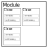
\includegraphics[width=8cm]{module.pdf}
  \end{center}
\end{figure}
\end{frame}

\begin{frame}[fragile]
Un fichier \textbf{\texttt{monmodule.py}} avec une classe \textbf{MaClasse}.

Dans un autre fichier:
  \begin{lstlisting}
    import monmodule
    
    objet = monmodule.MaClasse()
  \end{lstlisting}
\end{frame}

\begin{frame}[fragile]
Un fichier \textbf{\texttt{monmodule.py}} avec une classe \textbf{MaClasse}.

Dans un autre fichier:
  \begin{lstlisting}
    from monmodule import MaClasse
    
    objet = MaClasse()
  \end{lstlisting}
\end{frame}

\begin{frame}[fragile]
Un fichier \textbf{\texttt{monmodule.py}} avec une classe \textbf{MaClasse}.

Dans un autre fichier:
  \begin{lstlisting}
    from monmodule import MaClasse, MaClasse2
    
    objet = MaClasse()
  \end{lstlisting}
\end{frame}


\begin{frame}[fragile]
Un fichier \textbf{\texttt{monmodule.py}} avec une classe \textbf{MaClasse}.

Dans un autre fichier:
  \begin{lstlisting}
    from monmodule import *
    
    objet = MaClasse()
  \end{lstlisting}
\end{frame}

\section{Scripts \& Addons}
\begin{frame}
  \begin{itemize}
    \item Scripts : développement rapide
    \item Addons : ce qu'il faudra avoir à la fin
      \begin{itemize}
      \item Il faut ajouter des infos telles que nom, version, ...
      \end{itemize}

  \end{itemize}
\end{frame}


\begin{frame}[fragile]
  \frametitle{Addon = Module}
  \begin{lstlisting}
bl_info = {"name": "My Test Addon", "category": "Object"}
def register():
    print("Hello World")
def unregister():
    print("Goodbye World")
  \end{lstlisting}
\end{frame}

\begin{frame}[fragile]
  \frametitle{Du code simple...}
  \begin{lstlisting}
import bpy

scene = bpy.context.scene
for obj in scene.objects:
    obj.location.x += 1.0
  \end{lstlisting}
\end{frame}

\begin{frame}[fragile]
  \frametitle{...À l'addon}
  \begin{lstlisting}
bl_info = {
    "name": "Move X Axis",
    "category": "Object",
}

import bpy


class ObjectMoveX(bpy.types.Operator):
  \end{lstlisting}
\end{frame}

\begin{frame}[fragile]
  \begin{lstlisting}
class ObjectMoveX(bpy.types.Operator):
    """My Object Moving Script"""      # blender will use this as a tooltip for menu items and buttons.
    bl_idname = "object.move_x"        # unique identifier for buttons and menu items to reference.
    bl_label = "Move X by One"         # display name in the interface.
    bl_options = {'REGISTER', 'UNDO'}  # enable undo for the operator.

    def execute(self, context):        # execute() is called by blender when running the operator.

        # The original script
        scene = context.scene
        for obj in scene.objects:
            obj.location.x += 1.0

        return {'FINISHED'}            # this lets blender know the operator finished successfully.
  \end{lstlisting}
\end{frame}

\begin{frame}[fragile]
  \begin{lstlisting}

def register():
    bpy.utils.register_class(ObjectMoveX)


def unregister():
    bpy.utils.unregister_class(ObjectMoveX)


# This allows you to run the script directly from blenders text editor
# to test the addon without having to install it.
if __name__ == "__main__":
    register()
  \end{lstlisting}
\end{frame}

\section{Conventions de codage}
\begin{frame}
  \frametitle{Tabulations}
  {\Huge 4 espaces}
\end{frame}

\begin{frame}[fragile]
  \frametitle{Espaces}
  Opérateurs entourés d'espaces:
  \begin{lstlisting}[showspaces=true]
variable = 'valeur'
ceci == cela
1 + 2
  \end{lstlisting}
  
Non:
\begin{lstlisting}[showspaces=true]
variable='valeur'
ceci==cela
1+2
\end{lstlisting}
\end{frame}

\begin{frame}[fragile]
  \frametitle{Espaces}
  \textbf{Sauf...}
  
  \begin{itemize}
    \item Groupes d'expressions
    \begin{lstlisting}[showspaces=true]
a = x*2 - 1
b = x*x + y*y
c = (a+b) * (a-b)
\end{lstlisting}
    \item "=" dans les arguments d'une fonction
    \begin{lstlisting}[showspaces=true]
def fonction(arg='valeur'):
resultat = fonction(arg='valeur')
\end{lstlisting}
    \item parenthèses
    \begin{lstlisting}[showspaces=true]
2 * (3 + 4)
\end{lstlisting}
  \end{itemize}
\end{frame}

\begin{frame}[fragile]
  \frametitle{Noms de variables}
  Lettres uniquement, en minuscule:
  \begin{lstlisting}
for x in range(10):
    print(x)
 
i = get_index() + 12
print(ma_liste[i])
  \end{lstlisting}
  Underscores autorisés pour : modules, variables, fonctions et méthodes.
  
  \bigskip
  
  Pour les noms de classes: lettres uniquement, une majuscule par mot:
  \begin{lstlisting}
class CeciEstUneClasse:
    def methodiquement(self):
        pass
  \end{lstlisting}
\end{frame}


\section{Conclusion}
\begin{frame}
  \begin{itemize}
    \item RTM\\
          \url{http://www.blender.org/manual/}
    \item PEP-8\\
          http://sametmax.com/le-pep8-en-resume/
  \end{itemize}
\end{frame}
\end{document}
